\documentclass{lkx_paper}

\title{Cosmological Constraints from \\Baryonic Acoustic Oscillations}
\date{April 2025}
\author{Lev Kruglyak}

\lkxbib{final-paper}

\usepackage{graphicx}
\usepackage{float}

\renewcommand{\d}{{\mathrm{d}}}
\renewcommand{\b}{{\mathrm{b}}}
\renewcommand{\c}{{\mathrm{c}}}
\newcommand{\bc}{{\mathrm{bc}}}
\newcommand{\K}{{\mathrm{K}}}
\newcommand{\m}{{\mathrm{m}}}
\newcommand{\DE}{{\mathrm{DE}}}
\newcommand{\eff}{{\mathrm{eff}}}
\newcommand{\LCDM}{$\Lambda\mathrm{CDM}$~}

\DeclareMathOperator{\diag}{{\operatorname{diag}}}

\newcommand{\MM}{{\mathcal{M}}}
\newcommand{\DD}{{\mathcal{D}}}
\newcommand{\LL}{{\mathcal{L}}}
\usepackage{bm}
\newcommand{\pms}{{\bm{\theta}}}

\usepackage{siunitx}
\providecommand{\Mpcsi}[1]{\qty{#1}{\mathrm{Mpc}}}
\providecommand{\Hsi}[1]{\qty{#1}{\km\,\s^{-1}\,\mathrm{Mpc}^{-1}}}

\begin{document}

In this paper, we use measurements of baryon acoustic oscillation (BAO) measurements by the Dark Energy Spectroscopic Instrument (DESI) to obtain constraints on cosmological parameters in the \LCDM model.

\subsection*{The \LCDM Model}
We begin with a brief review of the \LCDM model and some of its variants.

Energy density is split into 6 species, baryonic matter $\Omega_\b$, cold (i.e. non-relativistic) dark matter $\Omega_\c$, electromagnetic radiation $\Omega_\gamma$, curvature $\Omega_\K$, neutrinos $\Omega_\nu$, and dark energy $\Omega_\DE$. Baryonic and cold dark matter is grouped as $\Omega_\bc=\Omega_\b+\Omega_\c$, while non-relativistic matter including neutrinos is grouped as $\Omega_\m=\Omega_\bc+\Omega_\m$.
Using standard equation of state parameters for $\Omega_\bc$, $\Omega_\gamma$, and $\Omega_K$, we can write the time-dependent Hubble parameter as:
\begin{equation}
  \frac{H(z)}{H_0} = 
  \left[\Omega_\bc(1+z)^3 + \Omega_\gamma(1+z)^4+\Omega_\K(1+z)^2+\Omega_\nu\frac{\rho_\nu(z)}{\rho_{\nu,0}} + \Omega_\DE \frac{\rho_\DE(z)}{\rho_{\DE,0}}\right]^{1/2}.
\end{equation}

\subsection*{Bayesian Analysis in Cosmology}

\subsection*{Results}
\begin{figure}[H]
  \centering
  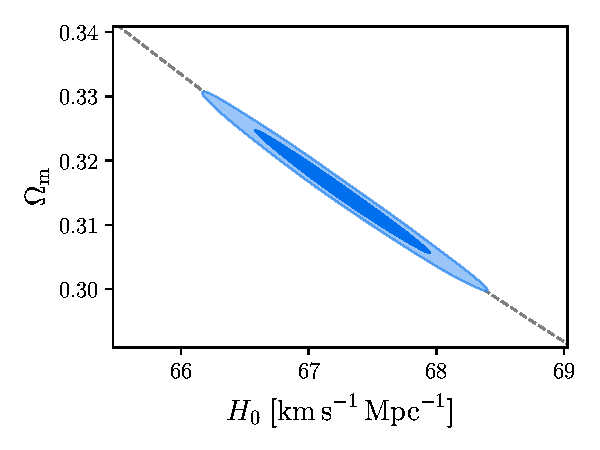
\includegraphics{figures/CMB-H0-omegam.pdf}
  \caption{}
\end{figure}

\cite{desicollaboration2025desidr2resultsii}

\end{document}
